\section[]{\selectlanguage{dutch} }
\clearpage\section[Werken met de grafische interface]{\foreignlanguage{dutch}{Werken met de grafische interface}}
\hypertarget{RefHeadingToc24621698778599}{}{\selectlanguage{dutch}
\foreignlanguage{dutch}{De Unix-wereld houdt erg van het paradigma ``Small is beautiful''. Daarmee bedoelen ze dat ze
graag kleine tools maken die \'e\'en ding goed doen. Dat zien we ook terug bij de grafische interface. Allereerst is er
een display server, dit is een stuk software dat ervoor zorgt dat er een grafische interface is. Het luistert naar de
muis en bestuurt de cursor en toont een grafisch scherm \ en dat is het wel zo'n beetje. Op deze grafische server
draait een window-manager. De window-manager vangt een applicatie in een frame (een window) en zorgt ervoor dat er naar
wens scrol-knoppen zijn en knopjes om het scherm te minimaliseren en/of te sluiten. Ook het achtergrondscherm is een
taak van de window-manager. Als laatste is er de desktop omgeving die zorgt voor de taakbalk, het configuratiescherm en
alle andere zaken die nodig zijn om van een desktop te kunnen spreken.}}

{\selectlanguage{dutch}
Als we dit allemaal hebben hebben we een desktop omgeving waarbinnen applicaties kunnen draaien.}

{\selectlanguage{dutch}
Er zijn twee dominante desktop omgevingen beschikbaar op de verschillende Linux distributies en dat zijn KDE en GNOME.
Naast deze twee zijn er nog vele verschillende anderen, maar die zullen we hier niet bespreken.}

{\selectlanguage{dutch}
\foreignlanguage{dutch}{KDE was de eerste van de twee genoemde desktopomgevingen en is gebaseerd op de Qt-library. In
het begin was de Qt-library geen open source vandaar dat er een concurrerent project is ontstaan. Later is het met Qt
helemaal goed gekomen en nu behoort ze tot de open source gemeenschap.}}

{\selectlanguage{dutch}
GNOME was het concurrerende project dat gestart werd omdat Qt niet open source was. Voor GNOME tot stand kwam was er een
open source fotomanipulatiepakket dat The \index{GIMP}GIMP heet, zie later in dit hoofdstuk. Om het pakket te kunnen
maken hadden de ontwikkelaars een grafische library ontwikkeld die GTK werd genoemd. Veel van wat er nodig is voor een
desktop zat daar al in en dus gebruikte het GNOME project de GTK-library als basis.}

{\selectlanguage{dutch}
\foreignlanguage{dutch}{De grafische interface kan enorm verschillen per distributie. Het maakt al enorm veel verschil
of je KDE of GNOME gebruikt als desktop omgeving. Laat je hierdoor niet imponeren, het wijst zich vaak vanzelf. KDE
ligt qua interface het dichtst tegen Windows aan, en zal dus het makkelijkst zijn om naar over te stappen. CentOS
gebruikt GNOME en vergt iets meer doorzettingsvermogen om te doorgronden.}}

{\selectlanguage{dutch}
\foreignlanguage{dutch}{Mocht het scherm in zijn screensaver vallen dan kan je door te clicken een scherm krijgen waarop
de tijd te zien is en met de {\textless}Enter{\textgreater} toets kom je op een login scherm en kan je in loggen met je
gebruikers wachtwoord.}}

{\selectlanguage{dutch}
\foreignlanguage{dutch}{Door op Activities te clicken krijg je extra scherm elementen te zien. Het nog een keer
aanclicken van Activities verbergt de elementen weer waardoor je meer ruimte op je scherm hebt voor applicaties.}}



\begin{center}
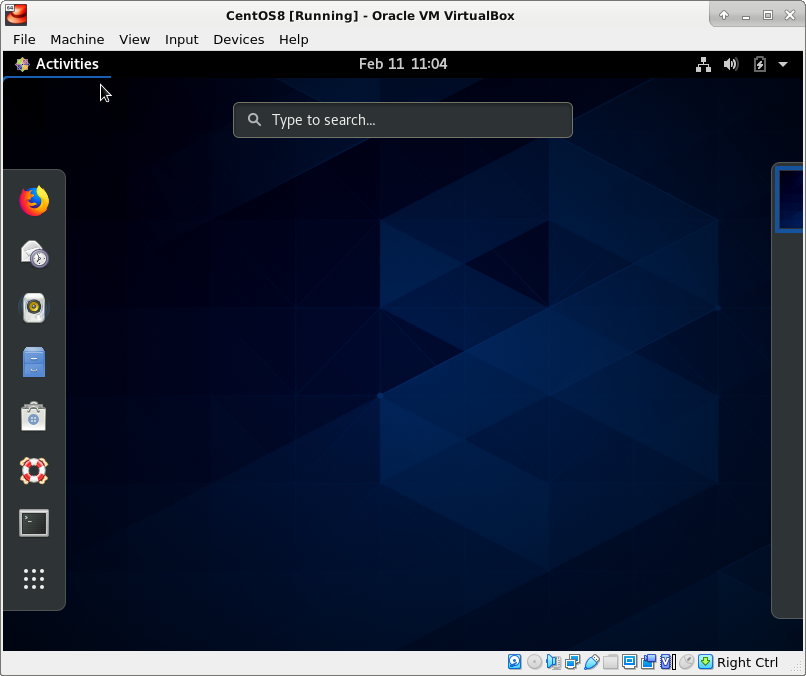
\includegraphics[width=3.1264in,height=2.6217in]{linuxreader-img013.png}
\end{center}
\begin{center}
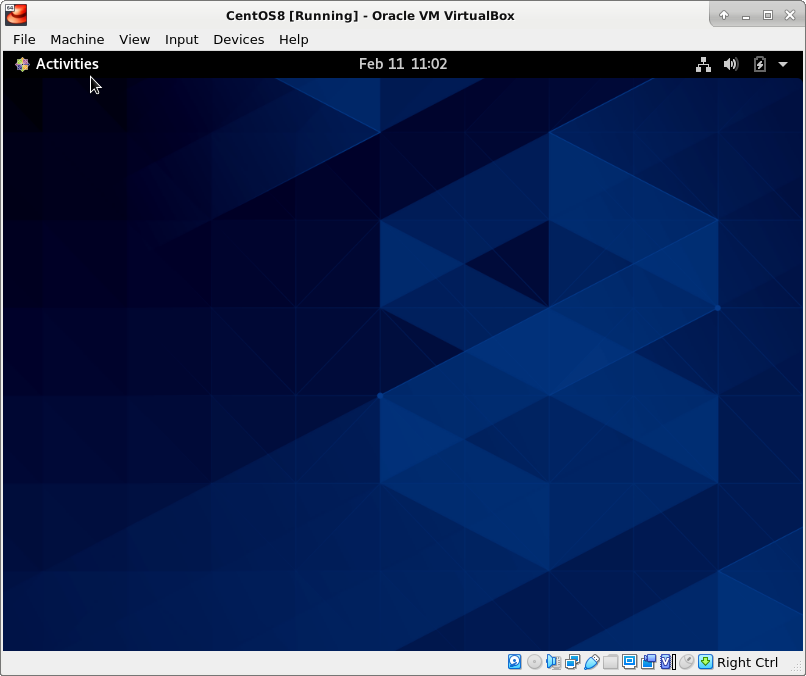
\includegraphics[width=3.1484in,height=2.6409in]{linuxreader-img014.png}
\end{center}

\bigskip

\subsection[Zoeken van bestanden of applicaties]{\selectlanguage{dutch} Zoeken van bestanden of applicaties}
\hypertarget{RefHeadingToc74801786672253}{}{\selectlanguage{dutch}
Met alle elementen op het scherm kan je de searchbar gebruiken om te zoeken op applicaties en bestanden. Als je zoekt op
Word, een Microsoft applicatie die niet op Linux beschikbaar is, dan vind je LibreOffice Writer een gratis en open
source alternatief. Start de applicatie op.}

{\selectlanguage{dutch}
Neem de tekst over van het plaatje hierboven en zorg dat dit een eerste hoofdstuk titel wordt door de stijl te
veranderen. We gaan het document later vullen. Selecteer File en Save as{\dots} om het bestand op te slaan als
Document1.}

\begin{center}
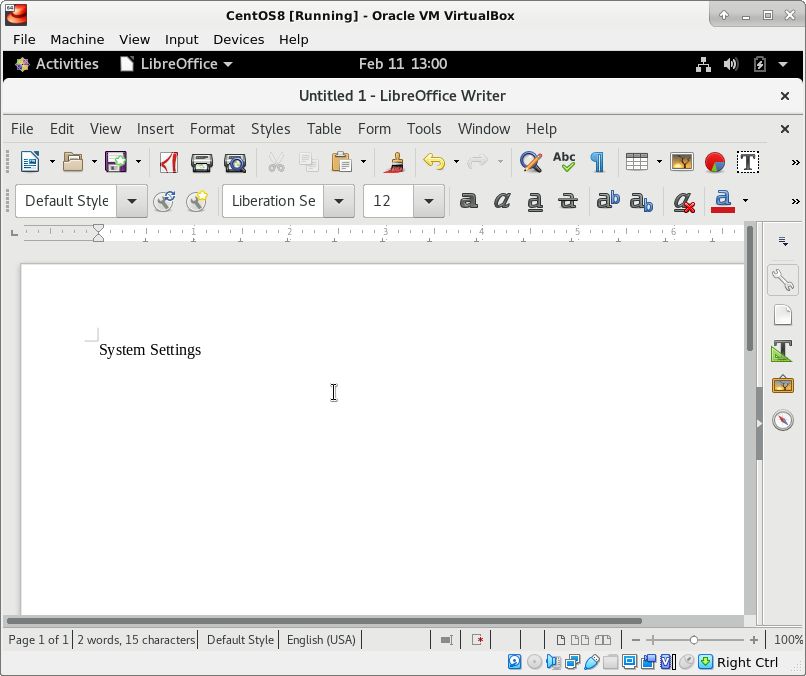
\includegraphics[width=4.8661in,height=4.0807in]{linuxreader-img015.png}
\end{center}
{\selectlanguage{dutch}
\foreignlanguage{dutch}{Meer over LibreOffice en de verschillende onderdelen van dit office pakket komt later aan de
orde als we Office Pakketten gaan bespreken. Nu concentreren we ons eerst op de beschikbare scherm elementen.}}

\subsection[Systeem configuratie]{\selectlanguage{dutch} Systeem configuratie}
\hypertarget{RefHeadingToc74821786672253}{}\index{Systeem configuratie}{\selectlanguage{dutch}
Op de donkere balk waarop ook Activities staat vind je aan de rechterkant een naar beneden wijzend driehoekje. Het
aanklikken van het driehoekje geeft een menu met daarop een overzicht van de helderheid van het scherm, aan welk
netwerk je gekoppeld bent, als je een laptop gebruikt wat de batterij status is, je loginnaam en drie knopjes die je
van links naar rechts toegang geven tot de systeemsettings, het locken van je scherm en het uitzetten of herstarten van
je machine.}



\begin{center}
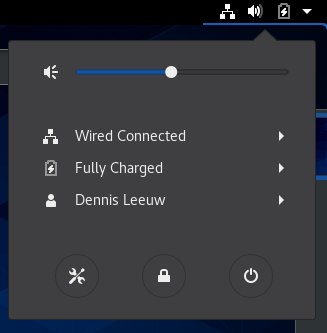
\includegraphics[width=2.2728in,height=2.3146in]{linuxreader-img016.png}
\end{center}
{\selectlanguage{dutch}
Selecteer Settings, scroll naar beneden naar Devices en selecteer deze, click dan op Displays. Trek het scherm los van
de topbar en schuif hem naar links. Click op de 800x600 resolutie en zet deze naar 1024x768}

{\selectlanguage{dutch}
\foreignlanguage{dutch}{Click op de Apply knop rechtsboven aan het scherm en daarna op Keep Settings. Natuurlijk mag je
resolutie ook hoger zetten, maar de minimale resolutie waarmee GNOME op CentOS 8 op een virtual machine prettig werkt
zonder dat je steeds met windows moet slepen is 1024x768. Selecteer {\textless} in de balk van Devices om terug te
komen in het hoofdmenu voor Settings. Loop door de verschillende opties om te ervaren waar je welke configuratie items
kan vinden en wijzigen.}}

\begin{center}
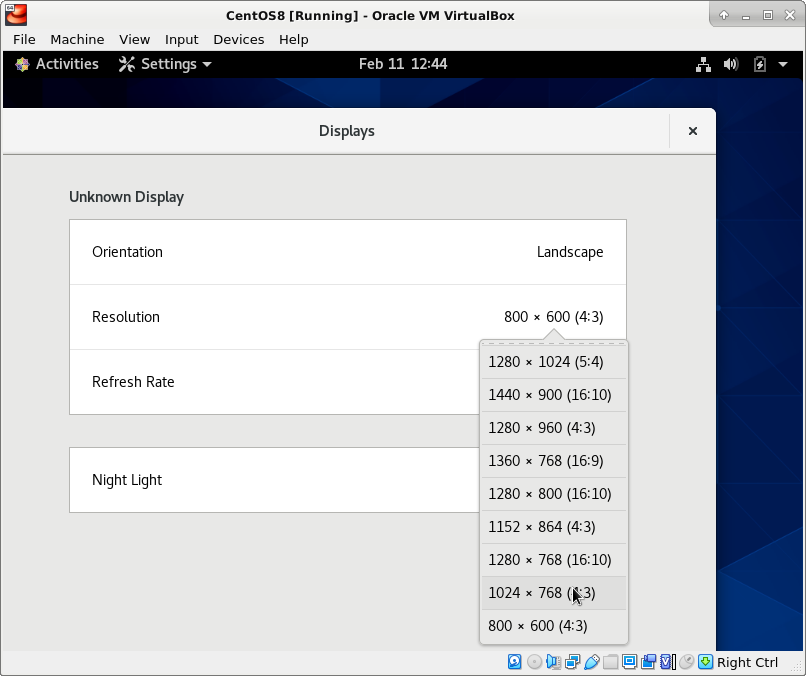
\includegraphics[width=5.089in,height=4.2681in]{linuxreader-img017.png}
\end{center}
{\selectlanguage{dutch}
\foreignlanguage{dutch}{[TODO] Opdracht met documentatie in Writer om iets op te zoeken en te documenteren in Document1.
}}


\bigskip

\subsection{The Dash}
\hypertarget{RefHeadingToc21382520829451}{}{\selectlanguage{dutch}
\ Aan de linkerkant van je scherm heb je de Dash, ook bekend als de Dock, applicatie bar of taskbar. Als je met je muis
over de iconen van de taskbar gaat dan zie je per icoon wat deze betekent. Van boven naar beneden kom je het volgende
tegen.}

\begin{center}
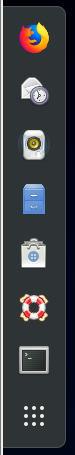
\includegraphics[width=0.7811in,height=4.7398in]{linuxreader-img018.png}
\end{center}
\liststyleLi
\begin{itemize}
\item {\selectlanguage{dutch}
Firefox -- een webbrowser}
\item {\selectlanguage{dutch}
Evolution -- Een e-mail client}
\item {\selectlanguage{dutch}
Rhythmbox -- een muziekspeler}
\item {\selectlanguage{dutch}
Files -- Bestandsbrowser}
\item {\selectlanguage{dutch}
Software -- Softwarebeheer}
\item {\selectlanguage{dutch}
Help -- Documentatie}
\item {\selectlanguage{dutch}
Terminal -- Toegang tot de console}
\item {\selectlanguage{dutch}
Show applications -- een beperkt overzicht van beschikbare applicaties.}
\end{itemize}
{\selectlanguage{dutch}
In de volgende hoofdstukken zullen we deze elementen doorlopen maar in een bredere context. We zullen bijvoorbeeld niet
alleen Firefox behandelen, maar webbrowsers in zijn algemeenheid.}

\subsection[Webbrowsers]{\selectlanguage{dutch} Webbrowsers}
\hypertarget{RefHeadingToc21402520829451}{}{\selectlanguage{dutch}
\foreignlanguage{dutch}{De meest gebruikte webbrowsers zijn Mozilla
}\index{Firefox}\foreignlanguage{dutch}{Firefox}\foreignlanguage{dutch}{, wat lange tijd de enige open source
webbrowser was op Linux. Het KDE-project heeft zijn eigen webbrowser ontwikkeld. Der KDE browser bestaat uit een engine
en en een interface. De engine is een library die alle benodigde functies voor het afhandelen van webpagina's heeft.
Het is ooit begonnen als KHTML. \ , de engine van deze browser,
}\index{WebKit}\foreignlanguage{dutch}{WebKit}\foreignlanguage{dutch}{ wordt inmiddels ook door Apple gebruikt voor
zijn Safari browser.}}

{\selectlanguage{dutch}
\foreignlanguage{dutch}{Toen Google zijn eigen webbrowser ontwikkelde werd de basis hiervan vrij gegeven als open source
browser met de naam }\index{Chromium}\foreignlanguage{dutch}{Chromium}\foreignlanguage{dutch}{. Google gebruikt zelf
ook deze basis voor zijn Chrome browser, maar voegt daar nog wat eigen elementen aan toe. De open source versie is ook
op Linux te gebruiken en wordt door veel distributies meegeleverd en is makkelijk later te installeren.}}

{\selectlanguage{dutch}
\foreignlanguage{dutch}{[TODO] Basisgebruik firefox}}

\subsection[E{}-mail clients]{E-mail clients}
\hypertarget{RefHeadingToc24521698778599}{}{\selectlanguage{dutch}
Mozilla levert naast de browser Firefox ook een open source \index{e-mail!e-mail client}e-mail client met de naam
\index{Thunderbird}Thunderbird dit is een volwaardige e-mail client inclusief kalenderfunctionaliteit.}

{\selectlanguage{dutch}
Een e-mail client die erg lijkt op Microsoft Outlook is \index{Evolution}Evolution. Sinds versie 2.8 is het onderdeel
van de GNOME project en Evolution is dan ook standaard ge\"installeerd op CentOS.}

{\selectlanguage{dutch}
Evolution en Thunderbird draaien ook op Windows en Mac OS X.}

{\selectlanguage{dutch}
Het KDE project heeft ook zijn eigen e-mail client en die heet \index{KMail}KMail. Standaard zijn er dus al vele e-mail
clients om uit te kiezen. Als je Op Internet gaat zoeken zijn er nog veel meer smaken beschikbaar. Dat is een van de
vele voordelen van open source, anderen zeggen een nadeel, er zijn enorm veel keuzes.}

{\selectlanguage{dutch}
[TODO] basis gebruik Evolution koppelen met google account (IMAP)}

\subsection[Office Pakketten]{\selectlanguage{dutch} Office Pakketten}
\hypertarget{RefHeadingToc24781698778599}{}{\selectlanguage{dutch}
\foreignlanguage{dutch}{Jaren lang was het meest gebruikte en dominante office pakket dat van Microsoft. Het was
beschikbaar voor Windows en Mac OS, maar niet voor Linux systemen. Oorspronkelijk had een Duitse student, Marco
B\"orries, StarWriter ontwikkeld om zijn studie in te documenteren. Later richtte hij een bedrijf op genaamd Star
Division en werd het een office pakket met de naam StarOffice. Het bedrijf werd in 1999 opgekocht door Sun Microsystems
die het pakket open source maakte onder de naam OpenOffice.org.}}

{\selectlanguage{dutch}
\foreignlanguage{dutch}{In 2009 werd Sun Microsystems gekocht door Oracle. Er was veel twijfel over wat Oracle met
OpenOffice.org wilde en dat zorgde voor een fork, een kopie van de code, die bekend werd onder de naam LibreOffice in
2010 en beheerd wordt door The Document Foundation. Oracle bracht }\foreignlanguage{dutch}{uiteindelijk in 2011 de code
van OpenOffice.org onder bij de Apache Foundation, helaas zat toen het merendeel van de ontwikkelaars al bij
LibreOffice. Beide projecten bestaan nog steeds, maar de meeste distributies leveren LibreOffice mee.}}

{\selectlanguage{dutch}
\foreignlanguage{dutch}{LibreOffice gebruikt standaard het Open Document Format voor al zijn documenten en is gratis
beschikbaar. Voor Linux, Mac OS X en Windows kan je het pakket vanaf de website downloaden
}\href{https://www.libreoffice.org/}{https://www.libreoffice.org}\foreignlanguage{dutch}{, maar dat hoeven wij niet te
doen omdat we het al meege\"installeerd hebben tijdens de installatie van CentOS.}}

{\selectlanguage{dutch}
LibreOffice bevat de volgende software onderdelen}

\liststyleLii
\begin{itemize}
\item {\selectlanguage{dutch}
Writer -- Tekstverwerking}
\item {\selectlanguage{dutch}
Calc -- Spreadsheets}
\item {\selectlanguage{dutch}
Impress -- Presentaties}
\item {\selectlanguage{dutch}
Draw -- Tekenpakket}
\item {\selectlanguage{dutch}
Math -- Een formule editor}
\item {\selectlanguage{dutch}
Base -- Database}
\end{itemize}
{\selectlanguage{dutch}
LibreOffice maakt standaard gebruik van het Open Document Format. Een officieel erkent en gestandaardiseerd
bestandsformaat dat er voor zorgt dat data altijd weer te lezen is omdat exact beschreven is hoe een document opgebouwd
moet zijn. De belangrijkste bestandsformaten zijn:}

\liststyleLiii
\begin{itemize}
\item {\selectlanguage{dutch}
odt -- Open Document Text}
\item {\selectlanguage{dutch}
ods -- Open Document Spreadsheet}
\item {\selectlanguage{dutch}
odp -- Open Document Presentation}
\item {\selectlanguage{dutch}
odi -- Open Document Image, bitmap format}
\item {\selectlanguage{dutch}
odg -- Open Document Graphic, vector format}
\item {\selectlanguage{dutch}
odf -- Open Document Formula}
\item {\selectlanguage{dutch}
odb -- Open Document Database}
\end{itemize}
\subsection[Grafische applicaties]{\selectlanguage{dutch} Grafische applicaties}
\hypertarget{RefHeadingToc21422520829451}{}\subsubsection[The Gimp]{\selectlanguage{dutch} The Gimp}
\hypertarget{RefHeadingToc24541698778599}{}\index{Gimp}{\selectlanguage{dutch}
De GIMP is een applicatie om foto's te bewerken. Je kan het vergelijken met Photoshop van Adobe. Voor diegene die gewend
zijn om te werken met Photoshop zal de interface aan de ene kant bekend voorkomen en aan de andere kant net even anders
zijn.}

\subsubsection[Inkscape]{\selectlanguage{dutch} Inkscape}
\hypertarget{RefHeadingToc24561698778599}{}{\selectlanguage{dutch}
\index{Inkscape}Inkscape is een applicatie om tekeningen in vectoren te maken. Het bouwt een tekening dus niet op in
pixels zoals bijvoorbeeld BMP, jpeg of PNG, maar doet dit door punten met vectoren te beschrijven, hierdoor zijn
tekeningen ``oneindig'' schaalbaar zonder kwaliteitsverlies.}

\subsection[Desktop publishing]{Desktop publishing}
\hypertarget{RefHeadingToc21442520829451}{}\subsubsection[Scribus]{\selectlanguage{dutch} Scribus}
\hypertarget{RefHeadingToc24581698778599}{}{\selectlanguage{dutch}
Een open source document opmaak pakket is \index{Scribus}Scribus. Het is vergelijkbaar met Adobe Pagemaker.}

\subsection[Multimedia Applicaties]{\selectlanguage{dutch}\sffamily Multimedia Applicaties}
\hypertarget{RefHeadingToc6804303847364}{}\subsubsection{Rhythmbox}
\hypertarget{RefHeadingToc6806303847364}{}\subsubsection{VLC}
\hypertarget{RefHeadingToc6808303847364}{}\subsubsection{KODI}
\hypertarget{RefHeadingToc6810303847364}{}\subsection[Bestandsbrowser]{Bestandsbrowser}
\hypertarget{RefHeadingToc6812303847364}{}\subsection[Installeren en updaten van software]{\selectlanguage{dutch}
Installeren en updaten van software}
\hypertarget{RefHeadingToc24861698778599}{}

\begin{center}
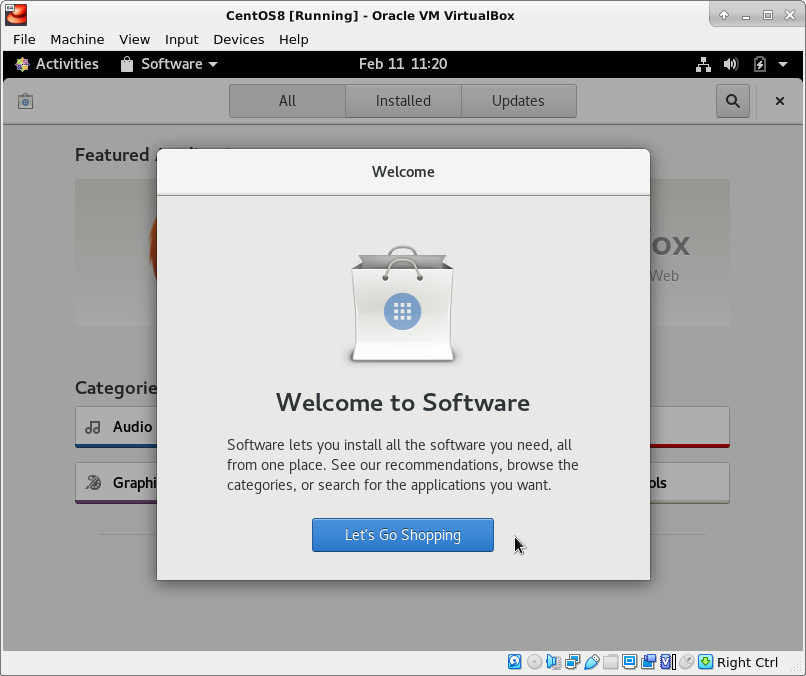
\includegraphics[width=6.9252in,height=5.8075in]{linuxreader-img019.png}
\end{center}
{\selectlanguage{dutch}
Rechtsboven kunnen we zoeken op een applicatie, we kunnen echter ook kiezen voor applicaties uit een Categorie. Klikken
we op Graphics \& Photography. Dan vinden we tussen de opties de Gimp. Selecteer de Gimp en klik Install. Er zal
gevraagd worden om het root-wachtwoord, na dit ingevoerd te hebben begint de installatie.}

{\selectlanguage{dutch}
Hierna kan je Software afsluiten of direct de Gimp opstarten.}

\begin{center}
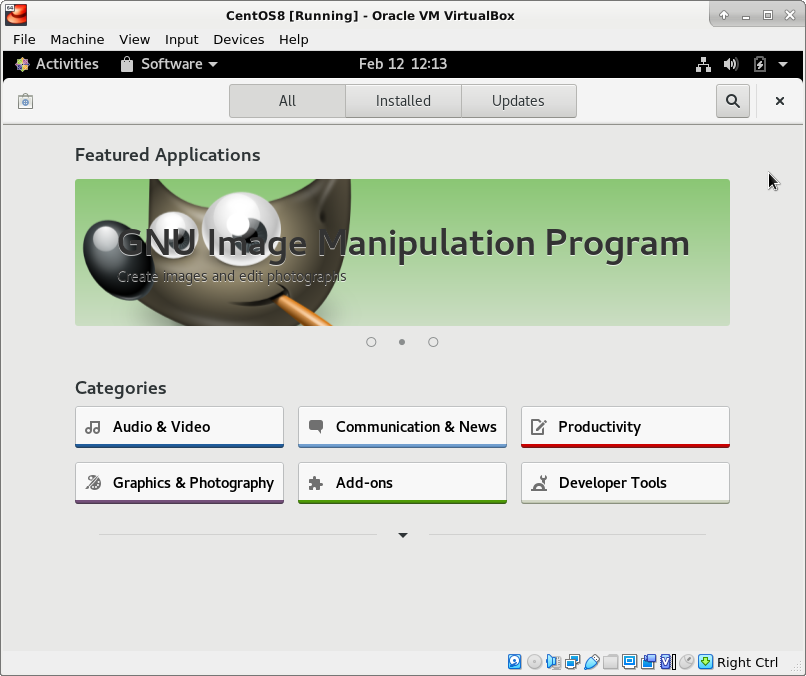
\includegraphics[width=6.9252in,height=5.8075in]{linuxreader-img020.png}
\end{center}
\subsection{Terminal}
\hypertarget{RefHeadingToc6814303847364}{}{\selectlanguage{dutch}
De terminal applicatie wordt gebruikt om op de command line terecht te komen. Deze applicatie komt later uitgebreid aan
de orde. Hier slaan we hem over.}

\subsection{Show Applications}
\hypertarget{RefHeadingToc6816303847364}{}{\selectlanguage{dutch}
Dit geeft een beperkt overzicht van de beschikbare applicaties. Voor snelle toegang tot de meest gebruikte applicaties
is dit een prima oplossing, verder is het makkelijker om gebruik te maken van de zoekfunctie zoals deze eerder in dit
document beschreven is.}

